\documentclass[a4paper,12pt,bibliography=totoc,numbers=noenddot]{scrartcl}\usepackage[]{graphicx}\usepackage[]{color}
%% maxwidth is the original width if it is less than linewidth
%% otherwise use linewidth (to make sure the graphics do not exceed the margin)
\makeatletter
\def\maxwidth{ %
  \ifdim\Gin@nat@width>\linewidth
    \linewidth
  \else
    \Gin@nat@width
  \fi
}
\makeatother

\definecolor{fgcolor}{rgb}{0.345, 0.345, 0.345}
\newcommand{\hlnum}[1]{\textcolor[rgb]{0.686,0.059,0.569}{#1}}%
\newcommand{\hlstr}[1]{\textcolor[rgb]{0.192,0.494,0.8}{#1}}%
\newcommand{\hlcom}[1]{\textcolor[rgb]{0.678,0.584,0.686}{\textit{#1}}}%
\newcommand{\hlopt}[1]{\textcolor[rgb]{0,0,0}{#1}}%
\newcommand{\hlstd}[1]{\textcolor[rgb]{0.345,0.345,0.345}{#1}}%
\newcommand{\hlkwa}[1]{\textcolor[rgb]{0.161,0.373,0.58}{\textbf{#1}}}%
\newcommand{\hlkwb}[1]{\textcolor[rgb]{0.69,0.353,0.396}{#1}}%
\newcommand{\hlkwc}[1]{\textcolor[rgb]{0.333,0.667,0.333}{#1}}%
\newcommand{\hlkwd}[1]{\textcolor[rgb]{0.737,0.353,0.396}{\textbf{#1}}}%

\usepackage{framed}
\makeatletter
\newenvironment{kframe}{%
 \def\at@end@of@kframe{}%
 \ifinner\ifhmode%
  \def\at@end@of@kframe{\end{minipage}}%
  \begin{minipage}{\columnwidth}%
 \fi\fi%
 \def\FrameCommand##1{\hskip\@totalleftmargin \hskip-\fboxsep
 \colorbox{shadecolor}{##1}\hskip-\fboxsep
     % There is no \\@totalrightmargin, so:
     \hskip-\linewidth \hskip-\@totalleftmargin \hskip\columnwidth}%
 \MakeFramed {\advance\hsize-\width
   \@totalleftmargin\z@ \linewidth\hsize
   \@setminipage}}%
 {\par\unskip\endMakeFramed%
 \at@end@of@kframe}
\makeatother

\definecolor{shadecolor}{rgb}{.97, .97, .97}
\definecolor{messagecolor}{rgb}{0, 0, 0}
\definecolor{warningcolor}{rgb}{1, 0, 1}
\definecolor{errorcolor}{rgb}{1, 0, 0}
\newenvironment{knitrout}{}{} % an empty environment to be redefined in TeX


\usepackage{alltt}
\usepackage[ngerman]{babel}
\usepackage{amsmath,amssymb}
\usepackage{enumerate}
\usepackage{blindtext}
\usepackage{listings}
%\usepackage{xcolor} % knitr automatically adds this
\usepackage{graphicx}
\usepackage{float}
\usepackage{rotating} % allows for rotation of tables
\usepackage{dcolumn} % aligns numbers regarding decimal point in tables
\usepackage{pdfpages}
\usepackage[onehalfspacing]{setspace}
\usepackage[left=3cm,right=2.5cm,top=2.5cm,bottom=2.5cm
  %,includeheadfoot
  ]{geometry}
\usepackage{varioref} % use \vref{} instead of \ref
\usepackage{pgf,tikz}
\usepackage[pdfborder={0 0 0}]{hyperref}
%\usepackage{apacite}
\usepackage{appendix}
\usepackage[T1]{fontenc}
\usepackage{lmodern}
\usepackage[utf8]{inputenc}
\usepackage[hybrid]{markdown}
\usepackage{url}
\usepackage[backend=biber,style=apa]{biblatex}
\DeclareLanguageMapping{german}{german-apa}
\usepackage[autostyle]{csquotes}
\addbibresource{References.bib}


\renewcommand{\familydefault}{\sfdefault}


%%%%%%%%%%%%%%% Define some commands: %%%%%%%%%%%%%%%%
\newcommand{\R}{\textrm{R}} % for correct writing of R, write \R

%%%%%%%%%%%%%%%%%%%%%%%%%%%%%%%%%%%%%%%%%%%%%%%%%%%%%%
%%%%%%%%%%%%%%% Check and edit this: %%%%%%%%%%%%%%%%%
%%%%%%%%%%%%%%%%%%%%%%%%%%%%%%%%%%%%%%%%%%%%%%%%%%%%%%
\newcommand{\theAuthor}{Tom Böger}
\newcommand{\theDate}{17. Oktober 2018}
\newcommand{\theAddress}{Bahnhofsstrasse 34}
\newcommand{\theZip}{9000}
\newcommand{\theCity}{St. Gallen}
\newcommand{\theMatriculation}{13-342-123}
\newcommand{\theTitle}{Dies ist der Haupttitel}
\newcommand{\theSubtitle}{Dies ist der Untertitel}
\newcommand{\theSupervisor}{Abgenommen von: Max Mustermann}
\newcommand{\theType}{Bachelorarbeit}
\newcommand{\theSemester}{Herbstsemester 2018}
%%%%%%%%%%%%%%%%%%%%%%%%%%%%%%%%%%%%%%%%%%%%%%%%%%%%%%

\labelformat{Kapitel}{section~#1}
\labelformat{Unterkapitel}{subsection~#1}
\labelformat{equation}{(#1)}
\labelformat{table}{table~#1}
\labelformat{Abbildung}{figure~#1}
% penalty for line break over pages
\clubpenalty = 10000
\widowpenalty = 10000

% Distance Toc-Title and first entry
\usepackage{tocloft}
%\setlength\cftaftertoctitleskip{30pt}
%%%%%%%%%%%%%%%%%%%%%%%%%%%%%%%%%%%%%%%%%%%%%%%%%%%%%%%%%%%%%%%%%%%%%%%%%%%%%%
\IfFileExists{upquote.sty}{\usepackage{upquote}}{}
\begin{document}

% Front page:
\begin{center}
\Large{
Universität St. Gallen\\
Hochschule für Wirtschafts-, Rechts- und Sozialwissenschaften (HSG)
}
\vspace{.9cm}
\hrule
\vspace{2.8cm}
\Huge{\textsf{\textbf{
\theTitle
}}}
\vspace{.5cm}

\Large{\textsf{\textbf{---\\ \theSubtitle}}}\\
\vspace{2.8cm}

\Large{\today}\\
\vspace{.9cm}

\Large{
\theAuthor\\
\theAddress\\
\theZip~\theCity\\
\theMatriculation}
\vspace{2cm}
\hrule
\vspace{.9cm}
\Large{\theType\\
\theSupervisor\\
\theSemester}
\end{center}
\thispagestyle{empty}


% Abstract:
%\newpage

\section*{Abstract}
\blindtext


\thispagestyle{empty}


\pagenumbering{Roman} % Change pagenumbering to capital roman numbers
% Preface:
%\newpage
\section*{Vorwort}
Dank an\dots

\blindtext


%%%%%%%%%%%%%%%%%%%%%%%%%%%%%%%%%%%%%%%%%%%%%%%%%%%%%%%%%%%%%%%%%%%%%%%%%%%%%%
%%%%%%%%%%%%%%%%%%%%%%%%%%%%%%%%%% Lists %%%%%%%%%%%%%%%%%%%%%%%%%%%%%%%%%%%%%
%%%%%%%%%%%%%%%%%%%%%%%%%%%%%%%%%%%%%%%%%%%%%%%%%%%%%%%%%%%%%%%%%%%%%%%%%%%%%%
% TOC
\newpage
\tableofcontents
\newpage
% Tabellenverzeichnis
%\phantomsection
%\addcontentsline{toc}{section}{Tabellenverzeichnis}
%\addtocontents{toc}{\protect\vspace{-5pt}}
%\listoftables
\newpage
% Abbildungsverzeichnis
%\phantomsection
%\addtocontents{toc}{\protect\vspace{-5pt}}
%\addcontentsline{toc}{section}{Abbildungsverzeichnis}
\listoffigures
%\lstlistoflistings

%%%%%%%%%%%%%%%%%%%%%%%%%%%%%%%%%%%%%%%%%%%%%%%%%%%%%%%%%%%%%%%%%%%%%%%%%%%%%%
% Load relevant things into R's memory, such as functions, data and packages %
%%%%%%%%%%%%%%%%%%%%%%%%%%%%%%%%%%%%%%%%%%%%%%%%%%%%%%%%%%%%%%%%%%%%%%%%%%%%%%

%%%%%%%%%%%%%%%%%%%%%%%%%%%%%%%%%%%%%%%%%%%%%%%%%%%%%%%%%%%%%%%%%%%%%%%%%%%%%%
%%%%%%%%%%%%%%%%%%%%%%%%%%%%%%%%% Content %%%%%%%%%%%%%%%%%%%%%%%%%%%%%%%%%%%%
%%%%%%%%%%%%%%%%%%%%%%%%%%%%%%%%%%%%%%%%%%%%%%%%%%%%%%%%%%%%%%%%%%%%%%%%%%%%%%
% Introduction:

\newpage
\pagenumbering{arabic}


\newpage
\markdownInput{markdown.md}
\newpage



% Conclusion:


% References
\newpage
\setlength{\bibitemsep}{.45\baselineskip}
\interlinepenalty=10000  %prevent splited bibitems
\printbibliography
%\bibliographystyle{apacite}
%\bibliography{References}
%%%%%%%%%%%%%%%%%%%%%%%%%%%%%%%%%%%%%%%%%%%%%%%%%%%%%%%%%%%%%%%%%%%%%%%%%%%%%%
%%%%%%%%%%%%%%%%%%%%%%%%%%%%%%%%%%% Appendix %%%%%%%%%%%%%%%%%%%%%%%%%%%%%%%%%
%%%%%%%%%%%%%%%%%%%%%%%%%%%%%%%%%%%%%%%%%%%%%%%%%%%%%%%%%%%%%%%%%%%%%%%%%%%%%%
\labelformat{section}{appendix~#1} % following sections are called appendix when refered to
\begin{appendices}
%\newpage
\section{Datendeklaration}
\blindtext

\newpage
\section{Anhang}
\begin{figure}[h]
    \centering
    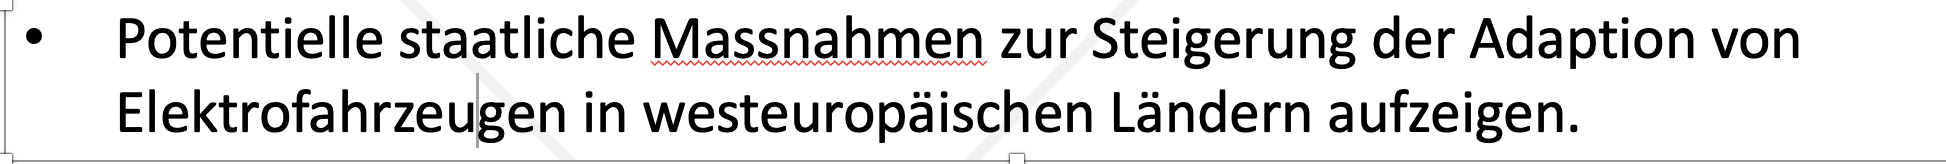
\includegraphics[width=0.4\textwidth]{figure/merge.png}
    \caption{Screenshots der Berner Zeitung und des Tagesanzeigers Online. Blau eingefärbt alle Artikel, die auf beiden Portalen platziert wurden. (Werbung entfernt, Abgerufen 4. Oktober 2018)}
    \label{}
\end{figure}

\end{appendices}

%%%%%%%%%%%%%%%%%%%%%%%%%%%%%%%%%%%%%%%%%%%%%%%%%%%%%%%%%%%%%%%%%%%%%%%%%%%%%%
%%%%%%%%%%%%%%%%%%%%%%%%%%%%%%% Academic Honesty %%%%%%%%%%%%%%%%%%%%%%%%%%%%%
%%%%%%%%%%%%%%%%%%%%%%%%%%%%%%%%%%%%%%%%%%%%%%%%%%%%%%%%%%%%%%%%%%%%%%%%%%%%%%
\section*{Eigenständigkeitserklärung}
Ich erkläre hiermit,
\begin{itemize}
\dass diese Hausarbeit von allen Mitgliedern des Teams mit gleichem Arbeitseinsatz und Engagement realisiert wurde, jedes Mitglied in gleichem Masse für das Ergebnis ver-antwortlich ist und über die Ergebnisse kompetent Auskunft geben kann;
\dass wir die vorliegende Arbeit selbstständig ohne fremde Hilfe (Lektorat, Überset-zungsdienstleister etc.) und ohne Verwendung anderer als der angegebenen Hilfsmittel verfasst haben;
\dass wir sämtliche verwendeten Quellen erwähnt und gemäss gängigen wissenschaftli-chen Zitierregeln (APA) korrekt zitiert haben;
\dass das Thema, die Arbeit oder Teile davon nicht bereits Gegenstand eines Leistungs-nachweises einer anderen Veranstaltung oder Kurses war (sofern dies nicht ausdrücklich mit dem/der Dozierenden im Voraus vereinbart wurde);
\dass unsere Arbeit mit allen Konsequenzen elektronisch auf Plagiate überprüft werden kann.
\end{itemize}
\vspace{1cm}
\hfill \theCity, \theDate
\\
\vspace{1.5cm}


\hfill \theAuthor
\thispagestyle{empty}


\end{document}
